\chapter{tempest program bug}
\label{sec:tempest_program_bug}
\lhead[tempest]{}
\lstset{style=6502Style}
There is more than one version of Tempest because some time after the game's
release in October 1981 players discovered a juicy little bug that hit arcade
owners where it hurts: in the pocketbook.

If you managed to reach a score of 170,000 or more there was a roughly one-in-eight chance that the next coin you
popped in the cabinet would give you a whopping forty credits to play with. The run-up
to Christmas was thoroughly ruined for Dave Theurer as this little heisenbug evolved
from impossible and easily-dismissed reports from arcade owners into something that the
Atari hardware technicians could reproduce in the lab. Theurer finally had to admit that
something was wrong somewhere, and it was probably his fault.



\begin{figure}[H]
    \centering
    \begin{adjustbox}{width=11cm,center}
      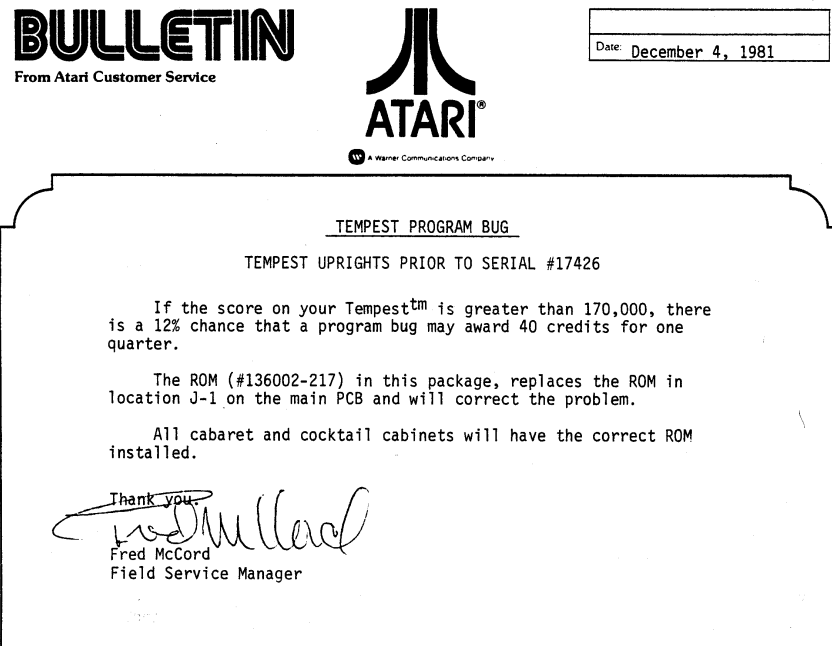
\includegraphics[width=12cm]{src/tempest_program_bug/bug.png}%
    \end{adjustbox}
  \caption{Field Service Bulletin December 1981.}
\end{figure}

Whatever the culprit was, the end result was that the number of credits available to the player was
magically inflated to 40 when they reached game over. So the only possible place to start is by first
looking at all the places that increment the variable responsible for storing credits. This is called
\icode{\$\$CRDT}, and like a lot of other variables, it lives in a region of memory known as the 'base page'.
Another common name for this region is the 'zero page'. This latter name gives us a hint about the region's location,
which starts at address zero. The first nine variables in Tempest's 'zero page' are given below. As you can see,
\icode{\$\$CRDT} is the seventh in the list, which means it has an address of \icode{\$06}.

\begin{lstlisting}
;
;CONTROL & TIMING VARIABLES
;
QSTATE:  .BLKB 1    ;CONTAINS CODE FOR STATE ROUTINE (INDEX INTO ROUTAD)
QDSTATE: .BLKB 1    ;DISPLAY STATE
QNXTSTA: .BLKB 1    ;NEXT STATE CODE TO EXECUTE AFTER PAUSE
QFRAME:  .BLKB 1    ;FRAME COUNTER (WRAPS AT FF)
QTMPAUS: .BLKB 1    ;PAUSE TIMER (IN SECOND UNITS)
QSTATUS: .BLKB 1    ;STATUS FLAGS
;
;OTHER OVERHEAD
;
$$CRDT:  .BLKB 1    ;# OF CREDITS
$INTCT:  .BLKB 1    ;INTERRUPT COUNT
$COINA:  .BLKB 1    ;COIN MECHS
\end{lstlisting}

We've gone to some pains to point this out because when we look at all the places where we increment \icode{\$\$CRDT} in the
Tempest codebase there really isn't anything that jumps out as unusual. The routines in \icode{COIN65.MAC} are responsible for
counting the coins inserted by the player. There is a very remote chance our problem is in here, but since it is common code used
by nearly all Atari titles we should only look there as a very last resort. We do find an interesting nugget in \icode{ALSCO2.MAC}, one
which explains the magic number of 40 reported by increasingly irate arcade managers:

\begin{lstlisting}
ZATC4C==ZATC4E-ZATC4S
        LDA $$CRDT    ; GET CURRENT CREDITS
        CMP I,28      ; IS IT MORE THAN HEX $28 (i.e. 40)?
        IFCS          ; IF SO THEN.. 
        LDA I,28      ; PUT 40 IN THE 'A' REGISTER
        STA $$CRDT    ; AND MAXIMIZE # CREDITS TO 40.
        ENDIF
\end{lstlisting}

The value in \icode{\$\$CRDT} is deliberately capped at 40, so the reason for this strangely specific number is because we are
clamping it to keep the number of credits at a reasonable limit. This means that more often than not the real number in \icode{\$\$CRDT}
is much higher and whatever is responsible for this
bug is incremementing it many times over. Since the maximum value we can store in a single byte is 255, and incrementing it beyond
that would result in it wrapping around to zero again, this starts to suggest to us that perhaps \icode{\$\$CRDT} is not being incremented
haphazardly, every now and then, but repeatedly and rapidly many times over, perhaps many times a second. This points us in the direction
of the code we run every time we paint a frame of the game. 

I think at this point in his investigation Dave Theurer might have started to get an inkling of where the problem was. The devious
mechanics we described in our copy protection chapter would have started to come back to him. Wasn't there something about writing
crazy values to the region of zero page memory when his code detected when a potential pirate had altered the appearance of any of the
game's screens? What was it we did again?

\begin{lstlisting}
ZQVAVG::
        LDA QT3     ; CHECK THAT BOTH QT3 AND
        ORA QT6     ; QT6 ARE ZERO.
        IFNE        ; IF THEY ARE NOT THEN
        LDA I,17    ; CHECK IF THE PLAYER' SCORE IS GREATER THAN 170,000
        CMP LSCORH  ; LSCORH CONTAINS THE FIRST 2 DIGITS OF THE PLAYER SCORE
        IFCC        ; IF IT IS GREATER THAN OR EQUAL TO 17..
        LDX LSCORL  ; LOAD WHATEVER IS IN THE LSCORL BYTE
        INC X,0     ; AND USE THAT TO INCREMENT ONE OF OUR 'ZERO-PAGE' BYTES.
        ENDIF       ; IN THE HOPE OF CAUSING SOME HAVOC.
        ENDIF       ; HAVOC SECURED.
\end{lstlisting}

A realization is beginning to dawn in the Tempest lab. We have discovered another magic number from the frantic bug reports. If the
score is at or above 170,000 (i.e. if the first two digits of the score are 17), we unleash a bit of havoc. Of course, we only do 
this if the checksums in \icode{QT3} or \icode{QT6} are non-zero. And this only happens if the screen content has been altered by
a third party. For example, if they have altered the copyright line to something else on the title screen. 

This would appear to be our smoking crater. If our copy-protection checks fail, and the player's score is 170,000 or above, we 
take the last two digits of their score from the byte \icode{LSCORL} and use that as index into the 'zero page' region of memory
to select a random variable to increment. So for example if the player's score is 172,004 we will increment the fifth byte in zero-page,
which is \icode{QTMPAUS}. If their score is 172,002 we will increment \icode{QDSTATE}. And if it is 172,006, or any value that ends with
a \icode{06}, we will increment our old friend \icode{\$\$CRDT}. We won't just increment it once and done - we'll increment it once every
frame, dozens of times a second. So it would appear that as long as you can score relatively highly and get your score ending with a
\icode{06} we will happily clock up your credits like billy-oh.

But of course for any of this to happen, the copy-protection has to fail. There's no good reason that should happen. Unless we forgot
to update the expected checksum values the last time we altered some screen content before shipping the game. We wouldn't have done
that, would we?

We take a look at the routine responsible for performing the copyright protection check.

\begin{lstlisting}
ZATVG2::
      LDA SECUVY      ; ARE WE DISPLAYING ONE OF THE TITLE SCREENS?
      IFNE            ; IF WE ARE THEN:
      LDY I,27        ; FOR ALL 39 BYTES IN THE VECTOR DISPLAYING THE ATARI COPYRIGHT
      LDA I,0E        ; STARTING FROM OUR HARD-CODE LITERAL OF '0E'
      SEC             ; CLEAR THE CARRY BIT SO IT DOESN'T INTERFERE
      ; LOOP THROUGH EACH CHARACTER IN THE LINE THAT CONTAINS '(C) MCMLXXX
      ; ATARI TO CALCULATE A FINAL CHECKSUM VALUE.
      BEGIN           ; LOOP FROM 27 TO 0
      SBC NY,SECUVG   ; SUBTRACT THE VALUE IN THE CURRENT CHARACTER FROM 'A'.
      DEY             ; DECREMENT Y TO GO TO THE PREVIOUS CHARACTER.
      MIEND           ; LOOP UNTIL Y IS 0.
      TAY             ; STORE THE RESULT IN A IN Y.
      IFNE            ; IF THE RESULT IS ZERO, THE CHECKSUM PASSES OTHERWISE:
      EOR I,0E5       ; CHECK IT AGAINST THE CHECKSUM FOR ANOTHER SCREEN
      ENDIF           
      IFNE            ; IF THAT PASSES WE'RE DONE OTHERWISE:
      EOR I,02A       ; CHECK IT AGAINST THE CHECKSUM FOR ANOTHER SCREEN
      ENDIF           
      STA QT3         ; STORE THE RESULT OF OUR CHECK IN QT3.
      ENDIF
      ENDIF
\end{lstlisting}

It comes back to us now. We iterate through all the characters on a particular line in the screen and use them to calculate
a primitive checksum. This is as simple as cumulatively subtracting the value of each byte on the line from an initial value
and checking that the result is what we expect. After a bit of pencil and paper testing we find that the first test passes:
the checksum on the high score screen results in a value of \icode{E5} in hex. We run the same test on the title screen
and discover our problem: the result is not \icode{2A}, it's \icode{29}. Oops.

Time to get on to Fred McCord and let him know he has a Christmas Field Service Bulletin to write and a bunch of replacement
ROMS to burn and package out to customers.


